%!TEX root=main.tex
\begin{section}{Introduction}
	\label{sec:intro}	
	\noindent Biomedical image analysis has been a natural area of application for deep convolutional neural networks (CNNs). Several uses of CNN-related topologies have been proposed in radiology\cite{Arbabshirani2018, Akkus2017}, histopathology \cite{ciresan2013, Litjens2016, Janowczyk2016} and microscopy \cite{Kraus2017, Sommer2017, Ciresan2012} (for a review, see \cite{Litjens2017}). High-content screening (HCS) \cite{Mattiazzi2016, Boutros2015, Singh2014, Scheeder2018, zock2009, assay2014}, the use of microscopy at scale in cellular experiments, in particular, has seen progress in applying CNN-based analysis \cite{Kraus2017, Godinez2017, Godinez2018, Sommer2017, Ando2017}. Instead of the conventional analysis approaches where cellular objects are first segmented and then pre-defined features representing their phenotypes (characteristic image content corresponding to the underlying experimental conditions) are measured, deep learning approaches offer the promise to capture relevant features and phenotypes without \textit{a priori} knowledge or significant manual parameter tuning. In deep CNNs, the deeper layers pick up high-levels of organization based on the input of many features captured in previous layers. Typically, a pooling operation (or a higher stride length in the convolution filter) is used to subsample interesting activations from one layer to the next, resulting in ever-coarser ``higher-level'' representations of the image content.\\\\
	\noindent Despite the potential of deep learning in analyzing biomedical images, two outstanding challenges, namely the complexity of the biological imaging phenotypes and the difficulty in acquiring large biological sample sizes, have hindered broader adoption in this domain. To circumvent these challenges, architectural changes have been introduced into some models to make training easier without trading off model accuracy. One novel approach is to use wide networks, which explicitly model various levels of coarseness. In these topologies, several copies of the input image are downsampled and used to train separate, parallel convolutional layers, which are eventually concatenated together to form a single feature vector that is passed on to fully-connected layers (e.g., see Buyssens et al.\cite{Buyssens2012}). A recent application of this idea to HCS is the Multiscale Convolutional Neural Network (M-CNN) architecture \cite{Godinez2017}, which has been shown to be generally applicable to multiple microscopy datasets, in particular for identifying the effect of compound treatment. \\\\
%	\begin{figure}[t]
%			\centering
%			\includegraphics[width=4.75in]{bbbc021_moa_examples_cropped.png}
%			\caption{\textsf{Cropped image regions highlighting phenotypes from the BBBC021\cite{bbbc021} dataset corresponding to treatments with compounds with different mechanisms of action: a) Microtubule destabilizer, b) DSMO (neutral control), c) Cholesterol lowering, d) Microtubule stabilizer,  e) Actin disrupter, f) Epithelial. See \autoref{fig:bbbc_whole} for the whole images. DNA staining is shown in blue, the F-actin staining in red and the Β-tubulin staining in green.}}
%			\label{fig:bbbc_cropped}
%	\end{figure}
\noindent The computational footprint of M-CNN, although relatively small as compared with other deep CNNs (e.g., Residual Neural Network 152), is still large when applied to high-content cellular imaging. Thus, it is important that model-related aspects of memory utilization and training performance are thoroughly understood, and that an end user knows \emph{a priori} how to get maximum performance on their hardware. Commercial cloud service providers (CSPs) like Microsoft, Google, or Amazon--as well as on-premise HPC centers in academia and industry--are exploring custom hardware accelerator architectures, such as application-specific integrated circuits (ASICs) \cite{jouppi2017} or GPUs, to expedite training neural network models. In spite of the popularity of these technologies, several factors such as higher financial cost of ownership, lack of virtualization and lack of support for multi-tenancy, leading to poor hardware utilization, may be cited as reasons to consider CPU-centric performance optimizations in reducing the time-to-train for such models. Importantly, since almost all data centers, are already equipped with thousands of general-purpose CPUs, it makes a strong case for such an approach. \\\\
\noindent Existing approaches to improve the time to train convolutional image classification neural network model such as M-CNN designed to work with large high-content cellular images have needed to either crop or down-sample the images during pre-processing. Other ideas are to restrict to small batch sizes or split the model across multiple devices due to the limited memory capacity available on GPUs or accelerator cards. However, these techniques can lead to longer time to convergence or time to train (TTT), and in some cases, lower model accuracy. CPUs, on the other hand, can leverage large memory. Our primary contributions include,

\begin{enumerate}
	\item Train M-CNN to achieve SOTA accuracy of 99\% on multiple CPU servers without tiling or cropping of input images or splitting the model
	\item Use large batch sizes per CPU exploiting large memory
	\item Use multiple training instances/workers per CPU node to improve utilization
	\item Use large batches and learning rate scaling to achieve fast convergence
\end{enumerate}

\noindent The ability to leverage large memory capacity on CPUs enables us to scale to larger batch sizes without having to crop or down-sample the input images. In conjunction with large batch sizes, we linearly scale learning rate with global batch size and train M-CNN to SOTA accuracy within one hour. We achieve this fast time to convergence using 128 two socket Intel® Xeon® 6148 processor nodes with 192GB DDR4 memory connected with 100Gbps Intel® Omnipath architecture.

	\begin{figure}[t]
	\centering
	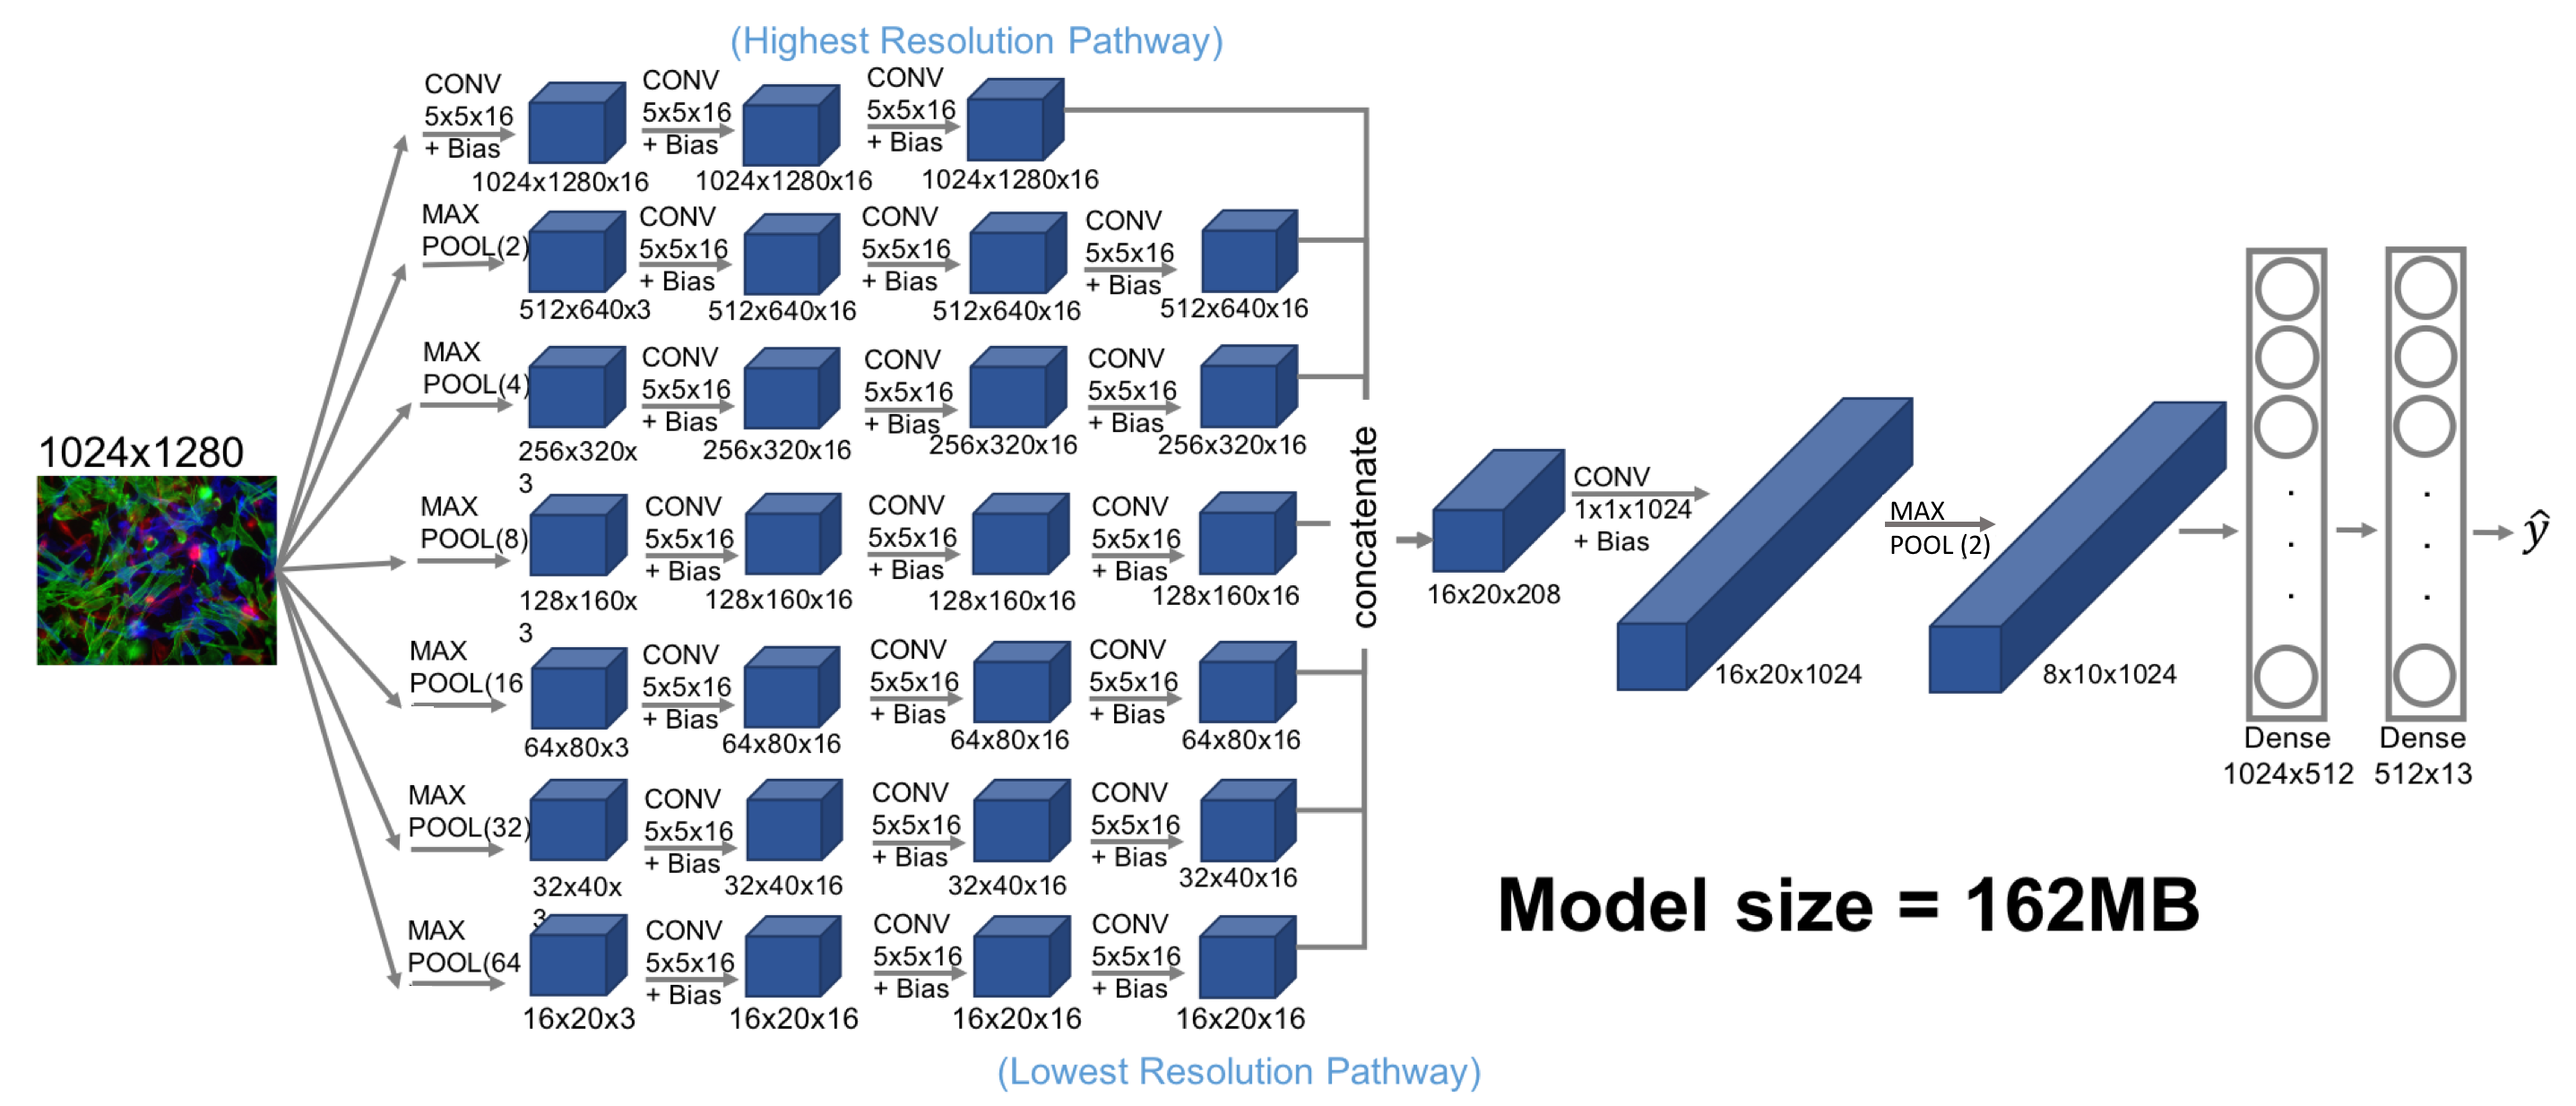
\includegraphics[width=4.75in]{mcnn.png}
	\caption{\textsf{Operations and kernels of the M-CNN model. Convolution is abbreviated \emph{CONV}, and Max Pooling operations are abbreviated as \emph{MAX POOL}}}
	\label{fig:mcnn}
\end{figure}

\end{section}



